\chapter{Stable stems, the image of \texorpdfstring{$J$}{J} and the Kervaire invariant}\label{ch:stable}

This chapter surveys what is known about the stable stems in the range where the Hopf maps are visible. Nothing here is new; the purpose is to state the results precisely, with their sources, and to separate the proved from the announced. Section~\ref{sec:parallel} contains the one elementary proof of the chapter.

\section{The stable stems through dimension nineteen}\label{sec:stems}

By Theorem~\ref{thm:freudenthal}, $\pi_k^s=\pi_{n+k}(S^n)$ for $n\ge k+2$. Table~\ref{tab:stable} lists $\pi_k^s$ for $k\le19$, after Toda \cite{Tod62} and Ravenel \cite[Table~A3.3]{Rav86}; the computations have since been extended far beyond this range by Isaksen, Wang and Xu \cite{IWX23}.

\begin{table}[ht]
\centering
\small
\begin{tabular}{@{}c|cccccccccc@{}}
\toprule
$k$ & $0$ & $1$ & $2$ & $3$ & $4$ & $5$ & $6$ & $7$ & $8$ & $9$\\
$\pi_k^s$ & $\Z$ & $2$ & $2$ & $24$ & $0$ & $0$ & $2$ & $240$ & $2^2$ & $2^3$\\
\midrule
$k$ & $10$ & $11$ & $12$ & $13$ & $14$ & $15$ & $16$ & $17$ & $18$ & $19$\\
$\pi_k^s$ & $6$ & $504$ & $0$ & $3$ & $2^2$ & $480{\oplus}2$ & $2^2$ & $2^4$ & $8{\oplus}2$ & $264{\oplus}2$\\
\bottomrule
\end{tabular}
\caption{The stable stems $\pi_k^s$ for $k\le19$ \cite{Tod62}, \cite[Table~A3.3]{Rav86}; an integer $m$ stands for $\Z/m$ and $2^j$ for $(\Z/2)^j$.}
\label{tab:stable}
\end{table}

The groups in degrees $1$, $3$ and $7$ are generated by the suspensions $\eta$, $\nu$, $\sigma$ of the three Hopf maps, and in degrees $2$, $6$ and $14$ the squares $\eta^2$, $\nu^2$ and $\sigma^2$ are nonzero \cite{Tod62}. The cyclic summands of orders $24$, $240$, $504$, $480$ and $264$ in degrees $3,7,11,15,19$ form the image of the $J$-homomorphism, described next.

\section{The \texorpdfstring{$J$}{J}-homomorphism}\label{sec:J}

An element of $\pi_k(\SO(n))$, represented by $\alpha\colon S^k\to\SO(n)$, defines a map $S^k\times S^{n-1}\to S^{n-1}$, $(x,v)\mapsto\alpha(x)v$, and the Hopf construction turns it into a map $S^{k+n}=S^k*S^{n-1}\to\Sigma S^{n-1}=S^n$. This defines Whitehead's homomorphism $J\colon\pi_k(\SO(n))\to\pi_{n+k}(S^n)$ \cite{Whi42}, compatible with suspension, and in the limit the stable homomorphism
\[
J\colon\pi_k(\SO)\to\pi_k^s .
\]
For $\K=\C,\Hq,\Oc$ the multiplication of unit vectors $S^{d-1}\times S^{d-1}\to S^{d-1}$ is the map associated with the clutching function $\tau$ of \eqref{eq:clutch}, and its Hopf construction is, up to homotopy and sign, the Hopf map $h_\K$; this is the classical link between the Hopf maps and $J$.

By Bott periodicity \cite{Bot59}, $\pi_k(\SO)$ for $k\ge1$ depends only on $k\bmod8$:
\[
\begin{array}{c|cccccccc}
k\bmod 8 & 0&1&2&3&4&5&6&7\\\hline
\pi_k(\SO) & \Z/2&\Z/2&0&\Z&0&0&0&\Z
\end{array}
\]

\begin{theorem}[Adams, Quillen, Sullivan, Becker--Gottlieb]\label{thm:imJ}
For $k\ge1$ the image of $J$ in $\pi_{4k-1}^s$ is a cyclic direct summand whose order is the denominator of $B_{2k}/4k$, where $B_{2k}$ is the Bernoulli number. For $k\ge1$ the image of $J$ in $\pi_{8k}^s$ and in $\pi_{8k+1}^s$ is $\Z/2$, and $J$ is injective on $\pi_{8k}(\SO)$ and $\pi_{8k+1}(\SO)$.
\end{theorem}

Adams \cite{Ada66} proved the lower bounds and the upper bound for the odd part, and reduced the rest to the \emph{Adams conjecture}: for a real vector bundle $\xi$ over a finite CW complex $X$ and an integer $\ell$, there is $e\ge0$ such that $\ell^e(\psi^\ell\xi-\xi)$ is fibre homotopy trivial, that is, maps to zero in $J(X)$, where $\psi^\ell$ is the Adams operation. The conjecture was proved by Quillen \cite{Qui71}, by Sullivan \cite{Sul74}, and by Becker and Gottlieb \cite{BG75}.\footnote{The statement of the conjecture in the earlier version of this work was garbled; the formulation here is that of \cite{Ada66}.}

\begin{table}[ht]
\centering
\small
\begin{tabular}{@{}c|cccccccccc@{}}
\toprule
$k$ & $1$ & $2$ & $3$ & $4$ & $5$ & $6$ & $7$ & $8$ & $9$ & $10$\\
\midrule
stem $4k-1$ & $3$ & $7$ & $11$ & $15$ & $19$ & $23$ & $27$ & $31$ & $35$ & $39$\\
$B_{2k}$ & $\frac16$ & $-\frac1{30}$ & $\frac1{42}$ & $-\frac1{30}$ & $\frac5{66}$ & $-\frac{691}{2730}$ & $\frac76$ & $-\frac{3617}{510}$ & $\frac{43867}{798}$ & $-\frac{174611}{330}$\\
$|\im J|$ & $24$ & $240$ & $504$ & $480$ & $264$ & $65520$ & $24$ & $16320$ & $28728$ & $13200$\\
\bottomrule
\end{tabular}
\caption{The order of the image of $J$ in $\pi_{4k-1}^s$, the denominator of $B_{2k}/4k$ (Theorem~\ref{thm:imJ}); the values are recomputed in Appendix~\ref{app:checks}.}
\label{tab:imJ}
\end{table}

\begin{remark}\label{rem:vonstaudt}
Write $m(2k)$ for the denominator of $B_{2k}/4k$. By the von Staudt--Clausen theorem the denominator of $B_{2k}$ is the product of the primes $p$ with $(p-1)\mid2k$, and for the other primes $B_{2k}/2k$ is $p$-integral (a consequence of the Kummer congruences). Hence
\[
m(2k)=2^{\,2+\nu_2(2k)}\prod_{p\ \mathrm{odd},\ (p-1)\mid 2k}p^{\,1+\nu_p(2k)},
\]
which gives $m(2)=2^3\cdot3=24$, $m(4)=2^4\cdot3\cdot5=240$, $m(6)=2^3\cdot3^2\cdot7=504$, $m(12)=2^4\cdot3^2\cdot5\cdot7\cdot13=65520$ and $m(14)=2^3\cdot3=24$. The formula is checked against Table~\ref{tab:imJ}, and against the Bernoulli numbers for $k\le60$, in Appendix~\ref{app:checks}.
\end{remark}

Figure~\ref{fig:imJ} shows the orders on a logarithmic scale.

\begin{figure}[ht]
\centering
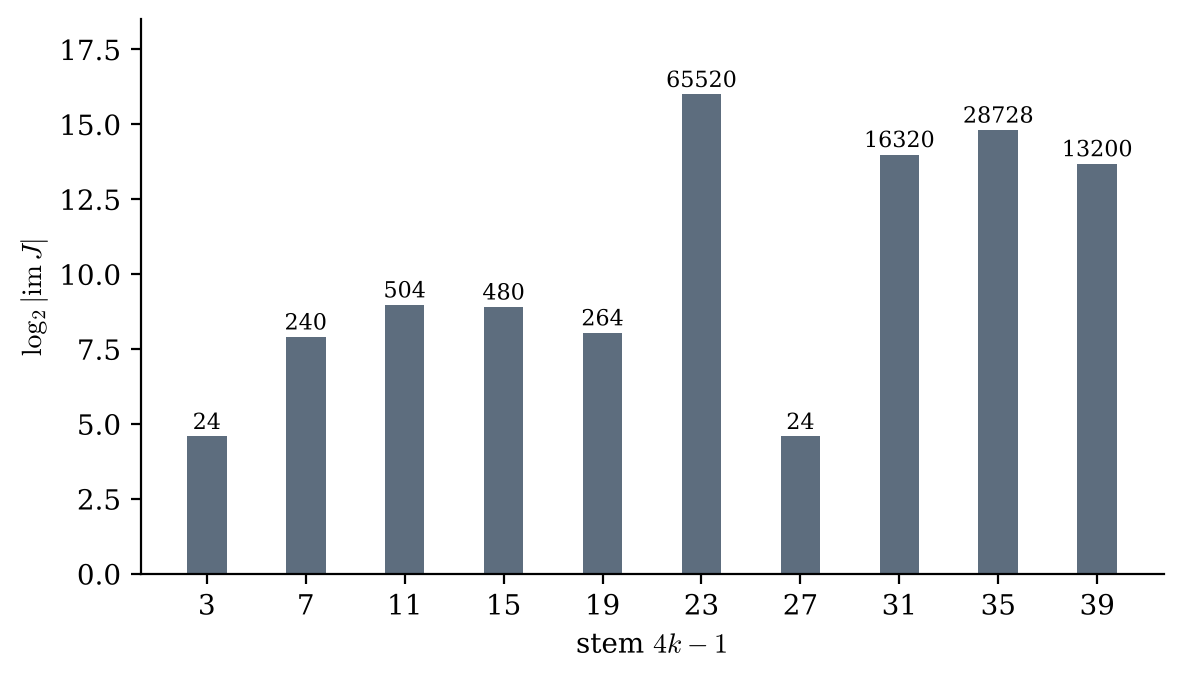
\includegraphics[width=0.85\textwidth]{fig_imageJ.png}
\caption{$\log_2|\im J|$ in the stems $4k-1$, $k=1,\dots,10$. The order is $24$ for $k=1$ and $k=7$, when $2$ and $3$ are the only primes $p$ with $(p-1)\mid2k$, and it is large when many such primes occur, as for $k=6$ (the primes $2,3,5,7,13$).}
\label{fig:imJ}
\end{figure}

\section{Division algebras and parallelisable spheres}\label{sec:parallel}

\begin{proposition}\label{prop:parallelisable}
The spheres $S^1$, $S^3$ and $S^7$ are parallelisable: if $e_1,\dots,e_{d-1}$ is an orthonormal basis of $\Imag\K$, then $x\mapsto xe_j$, $j=1,\dots,d-1$, are $d-1$ vector fields on $S^{d-1}$ that are orthonormal at every point.
\end{proposition}

\begin{proof}
By \ref{D:inner} and Lemma~\ref{lem:artin}, $\langle xa,xb\rangle=\langle a,\bar x(xb)\rangle=|x|^2\langle a,b\rangle$. For $|x|=1$ this gives $\langle xe_j,xe_k\rangle=\delta_{jk}$ and $\langle xe_j,x\rangle=\langle e_j,1\rangle=0$, so the vectors $xe_j$ are tangent to $S^{d-1}$ at $x$ and orthonormal.
\end{proof}

The converse is deep: $S^{n-1}$ is parallelisable only for $n=1,2,4,8$, by Bott--Milnor \cite{BM58} and Kervaire, and Adams determined the maximal number of linearly independent vector fields on every sphere \cite{Ada62}. Together with Corollary~\ref{cor:spherebundles} and Adams' theorem (I4), this is the topological form of the statement that $\R,\C,\Hq,\Oc$ are the only real normed division algebras.

\section{The Kervaire invariant}\label{sec:kervaire}

A framed manifold of dimension $4j+2$ has a Kervaire invariant in $\Z/2$, the Arf invariant of a quadratic refinement of its intersection form on middle-dimensional homology with $\Z/2$ coefficients; through the Pontryagin--Thom construction it becomes a homomorphism $\pi_{4j+2}^s\to\Z/2$. Browder proved that it vanishes unless the dimension has the form $2^{j+1}-2$ \cite{Bro69}. Let $\theta_j$ denote an element of Kervaire invariant one in $\pi_{2^{j+1}-2}^s$, when one exists.

\begin{theorem}\label{thm:kervaire}
\begin{enumerate}[label=\textup{(\roman*)}]
\item Elements $\theta_j$ exist for $j=1,2,3$, namely $\eta^2$, $\nu^2$ and $\sigma^2$, in the stems $2$, $6$ and $14$; for $j=4$ in stem $30$ \cite{BMT70}; and for $j=5$ in stem $62$ \cite{BJM84}.
\item No element $\theta_j$ exists for $j\ge7$, that is in the stems $254,510,\dots$ \cite{HHR16}.
\end{enumerate}
\end{theorem}

The only remaining case is $j=6$, the stem $126$. Lin, Wang and Xu \cite{LWX24} have announced a proof that $\theta_6$ exists; at the time of writing this is a preprint, and we record it as such. The first three cases show that the Hopf maps of the three non-commutative division algebras produce, through their squares, the first three elements of Kervaire invariant one.

\begin{remark}
Theorem~\ref{thm:kervaire} has a geometric meaning: for $j\neq6$ there is a closed smooth framed manifold of dimension $2^{j+1}-2$ with Kervaire invariant one exactly when $j\le5$ \cite{Bro69}, \cite{HHR16}.
\end{remark}
